\section{Resource Allocation and Sharing Algorithms}
\label{sc}
In this section we present two resource allocation algorithms and one resource sharing algorithm.

% \subsection{Multiple-Increase-Linear-Decrease(MILD)}

% Multiple-Increase-Linear-Decrease(MILD) is a algorithm used in medium access control for wireless LAN originally developed  in \cite{mild}. The original MILD algorithm is shown in equation \ref{mild_eq}. In equation \ref{mild_eq}, $x$ is the current back-off interval, $F_{inc}$ is the new back-off interval when a collision is detected, $F_{dec}$ is the new back-off interval if the current transmission is successful, $BO_{max}$ and $BO_{min}$ represent the upper and lower bound for the back-off interval value. 

% \begin{equation}
% \begin{aligned}
% \label{mild_eq}
% F_{inc}(x)&=Min(1.5x,BO_{max}) \\
% F_{dec}(x)&=Max(x-1,BO_{min})
% \end{aligned}
% \end{equation}

% The challenges Pacer resource allocation faces are similar to what medium access control for wireless LAN faces. First, collision in medium access control is analogous to a deadline miss in real-time application. Second, multiplicative increase of back-off interval upon a collision is analogous to multiplicative increase of CPU utilization when a deadline is missed in Pacer framework. Finally, linear decrease of back-off interval upon the current successful transmission is analogous to linear decrease of CPU utilization when the current heart rate does not miss the deadline  in Pacer framework.

% We modify MILD to fit Pacer resource allocation scheme. The new MILD algorithm are shown in equation \ref{mild_a_eq}, where $F$ is the CPU utilization assignment, $t$ is the time slot, $m$ and $n$ are parameters that satisfy $n>0$ and $1>m>0$, and $CU_{max}$ and $CU_{min}$ represent the upper and lower bound for CPU utilization value. We introduce two new parameters, $b_u$ and $b_l$, which are the upper bound and lower bound for acceptable heart rate respectively. The function of $b_u$ and $b_l$ is to define a range such that if a heart rate falls within this range, the CPU utilization remains constant, thereby achieves a smoother CPU utilization allocation curve when the algorithm reaches steady state. $m$ and $n$ can be tuned to achieve the desired performance. A large $m$ causes CPU utilization to decrease faster when heart rates are greater than $b_u$, but it can cause overshoot and make heart rates drop below the deadline. A small $n$ cause CPU utilization to increase faster when the heart rates are less than $b_l$, but it can cause overshoot and make heart rates greater than $b_u$.  To use AIMD algorithm, the user needs to specify $b_l$ and $b_u$, the upper and lower bound for heart rate. The AMID algorithm will adjust CPU utilization based on heartbeat feedback.


% \begin{equation}
% \begin{aligned}
% \label{mild_a_eq}
% F(t+1)=\left\{\begin{matrix}
% Min(1-F(t)*m,CU_{max})&\text{,if heart rate $> b_l$}\\
% x&\text{,if $b_u \geq$ heart rate $\geq b_l$} \\
% Max(F(t)-n,CU_{min})&\text{,if heart rate $<b_u$}
% \end{matrix}\right.
% \end{aligned}
% \end{equation}

\subsection{Additive-Increase-Multiplicative-Decrease(AIMD)}
AIMD\cite{aimd} is a popular feedback-based control algorithm. TCP congestion control is a well known use of AIMD, as shown in equation \ref{aimd_eq}, where $r$ is the sending rate, $t$ is the time slot, $m$ and $n$ are parameters that satisfy $m>0$ and $1>n>0$.
\begin{equation}
% \small
\label{aimd_eq}
r(t+1)=\left\{\begin{matrix}
\phantom{a}r(t)+m \quad \text{if congestion is not detected}\\
r(t)* n \quad \text{if congestion is detected} \quad
\end{matrix}\right.
\end{equation}

The challenges Pacer resource allocation faces are similar to what TCP control faces. First, congestion in TCP control is analogous to a deadline miss in real-time application. Second, additive increase of the sending rate before congestion occurs in TCP control is analogous to additive increase of spare CPU resources before a deadline miss in the Pacer framework. Finally, multiplicative decrease of transmission rate upon congestion is analogous to multiplicative decrease of spare CPU resources upon a deadline miss. 

We modify AIMD to fit the Pacer resource allocation scheme. The modified update rules for AIMD are shown in equation \ref{aimda1}, where $u(t)$ and $u(t+1)$ represent the current and the next CPU utilization assignment, $s(t)$ and $s(t+1)$ represent the current and next spared CPU utilization, $m$ and $n$ are parameters that satisfy $1>m>0$ and $1>n>0$. Operating on spare CPU resources instead of CPU resources directly ensures the demanded CPU utilization, $u(t+1)$, is always valid. In the modified AIMD, we also introduce two new parameters, $b_u$ and $b_l$, which are the upper bound and lower bound for acceptable heart rate value. The function of $b_u$ and $b_l$ is to define a range such that if a heart rate falls within this range, the CPU utilization demand remains constant, thereby achieves a smoother CPU utilization allocation curve when the algorithm reaches steady state. $m$ and $n$ can be tuned to achieve the desired performance. A larger $m$ causes CPU utilization to decrease faster when heart rates are greater than $b_u$, but it can cause overshoot and make heart rates drop below the lower bound, $b_l$. A smaller $n$ causes CPU utilization to increase faster when the heart rates are less than $b_l$, but it can cause overshoot and make heart rates greater than the upper bound, $b_u$. 

To use the AIMD algorithm, the developer needs to specify $m$, $n$, $b_l$ and $b_u$. The AIMD algorithm will adjust CPU utilization based on heartbeats feedback.

% \begin{equation}
% \label{aimda0}
% s(t)=1-u(t)
% \end{equation}

\begin{equation}
\begin{aligned}
\label{aimda1}
&s(t)=1-u(t)&&\\
&s(t+1)=\left\{\begin{matrix}
&s(t)+m \qquad &\text{if heart rate $> b_u$}\\
&s(t)&\text{if $b_u \geq$ heart rate $\geq b_l$} \\
&s(t)* n &\text{if heart rate $< b_l$ } 
\end{matrix}\right. \\
&u(t+1)=1-s(t+1)&&
\end{aligned}
\end{equation}

% \begin{equation}
% \label{aimda2}
% u(t+1)=1-s(t+1)
% \end{equation}


% We develop Additive-Decrease-Multiplicative-Increase(ADMI) that is inspired by Additive-Increase-Multiplicative-Decrease(AIMD)\cite{aimd}, a widely used feedback control algorithm. TCP congestion control is a well known implementation of AIMD, as shown in equation \ref{aimd_eq}, where $r$ is the sending rate, $t$ is the time slot, $m$ and $n$ are parameters that satisfy $m>0$ and $1>n>0$.
% \begin{equation}
% % \small
% \label{aimd_eq}
% r(t+1)=\left\{\begin{matrix}
% \phantom{a}r(t)+m \quad \text{if congestion is not present}\\
% r(t)* n \quad \text{if congestion is present} \quad
% \end{matrix}\right.
% \end{equation}

% The challenges Pacer resource allocation faces are similar what TCP control faces. First, congestion in TCP control is analogous to a deadline miss in Pacer framework. Second, additive increase of sending rate before congestion is detected in TCP control is analogous to additive decrease of CPU utilization before a deadline is missed in Pacer framework. Finally, multiplicative decrease of sending rate when a congestion is detected is analogous to multiplication increase of CPU utilization when a deadline is missed. 

% % We develop ADMI based on AIMD to fit Pacer resource allocation scheme. The update rules of ADMI are shown in equation \ref{aimd_a_eq}, where $u$ is the CPU utilization assignment, $t$ is the time slot, $m$ and $n$ are parameters that satisfy $m>0$ and $1>n>0$. Here, we introduce two new parameters, $b_u$ and $b_l$, which are the upper bound and lower bound for acceptable heart rate respectively. The function of $b_u$ and $b_l$ is to define a range such that if a heart rate falls within this range, the CPU utilization remains constant, thereby achieves a smoother CPU utilization allocation curve when the algorithm reaches steady state. $m$ and $n$ can be tuned to achieve the desired performance. A large $m$ causes CPU utilization to decrease faster when heart rates are greater than $b_u$, but it can cause overshoot and make heart rates drop below the deadline. A small $n$ cause CPU utilization to increase faster when the heart rates are less than $b_l$, but it can cause overshoot and make heart rates greater than $b_u$.  To use AIMD algorithm, the user needs to specify $b_l$ and $b_u$, the upper and lower bound for heart rate. The AMID algorithm will adjust CPU utilization based on heartbeat feedback.

% \begin{equation}
% \label{aimd_a_eq}
% u(t+1)=\left\{\begin{matrix}
% 1-(u(t)+m) \quad \text{if heart rate $\geq b_u$}\\
% u(t) \qquad \text{if $b_u \geq$ heart rate $\geq b_l$} \quad \\
% 1-u(t)* n \quad \text{if heart rate $\leq b_l$ } \quad 
% \end{matrix}\right.
% \end{equation}

\subsection{Self-Tuning Proportional-Integral-Derivative Control (STPID)}
STPID\cite{apid} is another feedback-based control algorithm. STPID's ability to adapt to system changes makes it a suitable resource allocation algorithm for applications with heterogeneous workloads. The block diagram STPID is shown in figure \ref{apid}, where $u$ is the target heart rate, $y_4$ is the feedback heart rate, and $e$ is the difference between $y_4$ and $u$. $\gamma$ in figure \ref{apid} is the parameter that dictates how sensitive the controller is to the error($e$ in figure \ref{apid}). We modify the algorithm such that $\gamma$ becomes an adaptive variable based on current error, $e$. The new update rule for $\gamma$ is shown in equation \ref{gamma}. With the new update rule, a larger $e$ gives a larger $\gamma$ which leads to a more aggressive response. 

To use the STPID controller, the developer just needs to specify $u$, the target heart rate. The STPID algorithm will adjust CPU utilization based on heartbeat feedback to reach the target heart rate.

\begin{equation}
\label{gamma}
\gamma =  \frac{log( \left | e \right |+1)}{log(u)}
\end{equation}

\begin{figure}[h!]
\centering
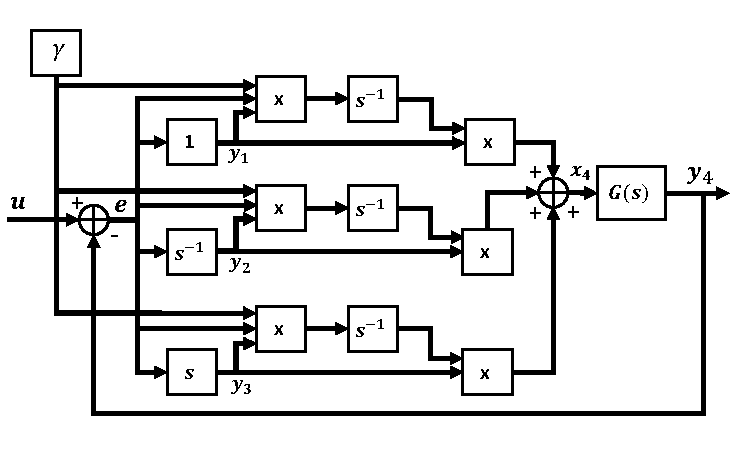
\includegraphics[width=1\linewidth]{images/apid}
\caption{Self-Tuning PID Controller\cite{apid}}
\label{apid}
\end{figure}

\subsection{Stride Sharing}
We develop a stride sharing algorithm that is inspired by stride scheduling\cite{stride}, a proportional-share CPU scheduler. Both stride sharing and stride scheduling distribute resources based on stride values. The major difference between stride scheduling and stride sharing is how the CPU resource is used. In stride scheduling, one particular task is selected to run with full CPU utilization for the current quantum while other tasks are put in a waiting queue. In stride sharing, a particular VM is selected to run with the CPU utilization it demands for current quantum while other VMs share the remaining CPU utilization instead of being inactive like the idle tasks in stride scheduling. The stride sharing algorithm is applied when the Pacer resource manager observes the total CPU utilization demand from the VMs exceeds the system's capacity. 

To use stride sharing, the developer needs to specify the stride values for the VMs that are sharing the same PCPU pool and the scheduling quantum that specifies the duration for the selected VM to run with the CPU resource it demands. AIMD and STPID can be used with stride sharing because AIMD and STPID calculate the CPU utilization each VM should request and stride sharing manages those requests when the system is oversubscribed.




